%
% $Id: SANDExampleReportstrict.tex,v 1.27 2009/04/30 23:15:05 rolf Exp $
%
% This is an example LaTeX file which uses the SANDreport class file.
% It shows how a SAND report should be formatted, what sections and
% elements it should contain, and how to use the SANDreport class.
% It uses the LaTeX report class and the strict option.
%
% Get the latest version of the class file and more at
%    http://www.cs.sandia.gov/~rolf/SANDreport
%
% This file and the SANDreport.cls file are based on information
% contained in "Guide to Preparing {SAND} Reports", Sand98-0730, edited
% by Tamara K. Locke, and the newer "Guide to Preparing SAND Reports and
% Other Communication Products", SAND2002-2068P.
% Please send corrections and suggestions for improvements to
% Rolf Riesen, Org. 9223, MS 1110, rolf@cs.sandia.gov
%
\documentclass[pdf,ps2pdf,12pt,report,strict,blank]{SANDreport}
\usepackage{hyperref}
\usepackage{multicol}
\usepackage{pslatex}
\usepackage{mathptmx}	% Use the Postscript Times font
\usepackage[FIGBOTCAP,normal,bf,tight]{subfigure}
\usepackage[dvips,light,first,bottomafter]{draftcopy}
\draftcopyName{Sample, contains no OUO}{70}

% If you want to relax some of the SAND98-0730 requirements, use the "relax"
% option. It adds spaces and boldface in the table of contents, and does not
% force the page layout sizes.
% e.g. \documentclass[relax,12pt]{SANDreport}
%
% You can also use the "strict" option, which applies even more of the
% SAND98-0730 guidelines. It gets rid of section numbers which are often
% useful; e.g. \documentclass[strict]{SANDreport}



% ---------------------------------------------------------------------------- %
%
% Set the title, author, and date
%
    \title{Optika: A GUI Framework for Parametrized Applications (Report style, strict)}

    \author{Kurtis L. Nusbaum \\
	  Scalable Algorithms \\
	  Sandia National Laboratories\\
	  P.O. Box 5800\\
	  Albuquerque, NM 87185-9999 \\
	  klnusba@sandia.gov \\
	 }

    % There is a "Printed" date on the title page of a SAND report, so
    % the generic \date should generally be empty.
    \date{}


% ---------------------------------------------------------------------------- %
% Set some things we need for SAND reports. These are mandatory
%
\SANDnum{SAND2010-xxxx}
\SANDprintDate{July 2010}
\SANDrePrintDate{January 2006}
\SANDrePrintDate{February 2006}
\SANDrePrintDate{March 2006}
\SANDauthor{Kurtis L. Nusbaum}


% ---------------------------------------------------------------------------- %
% Include the markings required for your SAND report. The default is "Unlimited
% Release". You may have to edit the file included here, or create your own
% (see the examples provided).
%
% \include{MarkUR} % Not needed for unlimted release reports


% ---------------------------------------------------------------------------- %
% The following definition does not have a default value and will not
% print anything, if not defined
%
\SANDsupersed{SAND1901-0001}{January 1901}


% ---------------------------------------------------------------------------- %
%
% Start the document
%
\begin{document}
    \maketitle

    % ------------------------------------------------------------------------ %
    % An Abstract is required for SAND reports
    %
    \begin{abstract}
	In the field of scientific computing there are many specialized programs designed for specific applications 
in areas like biology, chemistry, and physics. These applications are often very powerful and extraodinarily 
useful in their respective domains. However, many suffer from a common problem: a non-intutive, poorly designed user interface. Many 
of these programs are homegrown, and the concern of the designer was not ease of use but rather 
functionality. The purpose of Optika is to address this problem and provide a simple, viable solution. Using
only a list of parameters passed to it, Optika can dynamically generate a GUI. This allows the user to specify 
parameter's values in a fashion that is much more intuitive than the traditional "input decks" used by many 
parameterized scientific applications. By leverageing the power of Optika, these scientific applications 
will become more accessible and thus allow their designers to reach a much wider audience while requiring 
minimal extra development effort.

    \end{abstract}


    % ------------------------------------------------------------------------ %
    % An Acknowledgement section is optional but important, if someone made
    % contributions or helped beyond the normal part of a work assignment.
    % Use \section* since we don't want it in the table of context
    %
    \clearpage
    \chapter*{Acknowledgment}
	    Thanks to Dr. Mike Heroux and Jim Willenbring. Their mentoring
	has been crucial to the development of Optika. Also, many thanks
	to the entire Trilinos Community in which Optika has found a
	welcoming home.

    The format of this report is based on information found
    in~\cite{Sand98-0730}.



    % ------------------------------------------------------------------------ %
    % The table of contents and list of figures and tables
    % Comment out \listoffigures and \listoftables if there are no
    % figures or tables. Make sure this starts on an odd numbered page
    %
    \cleardoublepage		% TOC needs to start on an odd page
    \tableofcontents
    \listoffigures
    \listoftables


    % ---------------------------------------------------------------------- %
    % An optional preface or Foreword
    %\clearpage
    %\chapter*{Preface}
    %\addcontentsline{toc}{chapter}{Preface}
	%    Although staff members usually have only limited experience
    with dry-erase markers, and many even dispute their existence,
    it is worthwhile to be open minded and explore the possibilities.



    % ---------------------------------------------------------------------- %
    % An optional executive summary
    %\clearpage
    %\chapter*{Summary}
    %\addcontentsline{toc}{chapter}{Summary}
	%    Once a certain level of mistrust and skepticism has been
    overcome, dry-erase markers find many uses in todays science and
    engineering. In this report we explain some of the fundamental
    properties, dangers, and benefits of dry-erase markers. We then
    conclude with a few examples on how they can be used in daily
    activities at national Laboratories.



    % ---------------------------------------------------------------------- %
    % An optional glossary. We don't want it to be numbered
    \clearpage
    \chapter*{Nomenclature}
    \addcontentsline{toc}{chapter}{Nomenclature}
    \begin{description}
	\item[Dependency]
	    A relationship ship between to parameters in which the state
		or value of one parameter depends on the state or value of
		another.
	\item[Dependee]
		The parameter upon which another parameter state or value dependes.
	\item[Dependent]
		A parameter whose state or value is determined by another
		parameter.
	\item[Parameter]
	    An input needed for a program.
	\item[Parameter List]
	    A list of parameters and other parameter lists.
	\item[RCP]
	    Refernce counted pointer. RCPs refered to in this document reference the
		RCP class located in the Teuchos package of Trilinos.
	\item[Sublist]
	    A parameter list contained within another parameter list.
	\item[Widget]
		A GUI element, usually used to obtain user input.
	\item[Validator]
		An object used to ensure a particular parameter's value is valid.
    \end{description}


    % ---------------------------------------------------------------------- %
    % This is where the body of the report begins; usually with an Introduction
    %
    \SANDmain		% Start the main part of the report

    \chapter{Introduction}
	\label{Intro}
	\section{Introduction}
In the world of scientific computing there is a problem: most software developers are far more concerned
with the functionality of their software rather than their user interface. This is understandable given
the limited time and pressures of scientific computing environments. And in 
cases where there are only a few users of a piece of software this type of development is tolerable. However, when a piece of
software starts to be used by a wider audience, poor user interface design issues come to the forefront and 
can greatly hinder further adoption of a particular piece of software. Optika\footnote{For more information on Optika, please see
its documentation~\cite{OptikaPackage}} is an attempt to solve this
problem in a generic fashion for parameterized scientific applications.

Since developers of scientific applications don't really care about user interfaces, Optika needs
to provide a minimal amount of hurdles for developers. Also, the end result needs to be an intuitive
user interface that can be easily navigated and utilized regardless of the underlying computations being done.

The purpose of this paper is to discuss the development of the Optika package. In doing so we hope to
demonstrate how Optika solved some of the issues associated with developing a generic user interface
for scientific applications and provide justification for why we chose particular solutions. We will
proceed to discuss Optika development in a semi-chronological fashion.




    \chapter{Development of the Optika package}
	This section of the report discusses the developement of the Optika package.
	\section{Initial Planning and Development}
In Fall of 2008, Dr. Mike Heroux identified a need for
the Trilinos Framework\footnote{Optika is part of the Trilinos Project~\cite{1089021}.} to include some sort of GUI package. Dr. Heroux wanted 
to give users of the framework the ability to easily generate GUIs for their
programs, while still providing a good experience for the end-user. Based on
previous GUI work we'd done for the Tramonto project~\cite{Tramonto}, a few initial problems were
identified:

	\begin{itemize}
		\item How would the GUI be laid out?
		\item What GUI framework would would be used to build the GUI?
		\item Different types of parameters require different methods of input.
			How would the program decide how to obtain input for a particular
			parameter?
		\item How would the application developer specify parameters for the
			GUI to obtain?
		\item How would the application developer specify dependencies between
		parameters. This was a crucial problem/needed-feature that was identified in
		previous development of an unsuccessful Tramonto GUI.
	\end{itemize}

After some deliberation, the following initial solutions were decided upon:

	\begin{itemize}
		\item The GUI would be laid out in a hierarchical fashion as shown in
		Figure \ref{paramlistFigure}. Parameters would be organized into lists and sublists. This
		would allow for a clear organization of the parameters as well as
		intrinsically demonstrate the relationships between them.
		\begin{figure}
			\centering
			\begin{picture}(50,150)(0,0)
				\put(10,0){\line(0,1){145}}
				\put(0,150){${Parameter List}$}
				\put(10,130){\line(1,0){15}}
				\put(28,127){$Parameter$}
				\put(10,110){\line(1,0){15}}
				\put(28,107){$Parameter$}
				\put(10,90){\line(1,0){15}}
				\put(28,87){$Parameter$}
				\put(10,70){\line(1,0){15}}
				\put(28,67){$Parameter List$}
				\put(38,0){\line(0,1){62}}
				\put(38,47){\line(1,0){15}}
				\put(56,44){$Parameter$}
				\put(38,22){\line(1,0){15}}
				\put(56,24){$Parameter$}
			\end{picture}
			\caption[GUI Layout]{The hierarchical layout of the GUI}
			\label{paramlistFigure}
		\end{figure}
		\item QT\footnote{For documentation on all Qt classes please visit~\cite{QtDocs}.} was chosen as the GUI framework for several reasons:
			\begin{itemize}
				\item It is cross-platform.
				\item It is mature and has a comprehensive set of
				development tools.
				\item It has a rich feature-set.
				\item It has been used by Sandia in the past.
				\item The Optika lead developer was familiar with it.
			\end{itemize}
		\item It would be required that all parameters specify their type and the
		following types would be accepted:
			\begin{multicols}{2}
			\begin{itemize}
				\item int
				\item short
				\item float
				\item double
				\item string
				\item boolean
				\item arrays of int, short, double, and string
			\end{itemize}
			\end{multicols}
		The supported data type were chosen for two main reasons:
		\begin{inparaenum}[(a)]
			\item The number of input widgets that need to be supported
			is a direct function of the supported data types. By only supporting
			a small set of basic data types, we could stick
			to supporting only a small number of input widgets, most of which
			were already pre-built and part of Qt.
			\item The development team felt that these data types would be
			adequate for 95\% of the developers who would be using Optika.
		\end{inparaenum}

		For number types, a spin box (figure~\ref{spinboxfig}) would be used as input. If the valid
		values for a string type were specified, a combo box (figure~\ref{comboboxfig}) would be used.
		Otherwise a line edit (figure~\ref{lineeditfig}) would be used. For booleans, a combo box (figure~\ref{comboboxfig}) would
		also be used. For arrays, a pop-up box containing numerous input
		widgets would be used. The widget type would be determined by the
		array type (e.g. for numerical types a series of spinboxes would be used). 
		\begin{figure}[h]
			\centering
			\subfigure[A Spin Box]{
				\label{spinboxfig}
				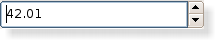
\includegraphics[scale=0.5]{graphics/spinbox}
			}
			\subfigure[A Combo Box]{
				\label{comboboxfig}
				
\includegraphics[scale=0.5]{graphics/combobox}
			}
			\subfigure[A Line Edit]{
				\label{lineeditfig}
				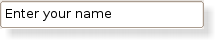
\includegraphics[scale=0.5]{graphics/lineedit}
			}
			\caption{Some of the various widgets used for editing data~\cite{QtGallery}}
			\label{editingWidgets}
		\end{figure}

		\item Initially it was decided that the application developer would
		specify parameters via an XML file. A DTD would be created specifying
		the legal tags and namespaces.
		\item Dependencies would be handled through special tags in the DTD.
	\end{itemize}

\section{Early Development}
The first several months of development were spent on creating and implementing the XML
specification. The name of the XML specification went through several revisions but was
eventually called Dependent Parameter Markup Language (DPML).

After several months of development we realized that creating an entirely new way of specifying 
parameters might hinder adoption of Optika. We also realized that Trilinos actually had
a ParameterList class in the Teuchos~\cite{TeuchosPackage} package. The ParameterList seemed to be better than DPML for
several reasons:
	\begin{itemize}
		\item It was already heavily adopted.
		\item It had the necessary hierarchical nature (like described in figure~\ref{paramlistFigure}).
		\item It was serializable to and from XML.
	\end{itemize}

For these reasons, DPML was scrapped in favor of using Teucho's ParameterLists. Development moved
forward with the goal of creating a GUI framework that, in addition to meeting all the challenges 
outlined above, would also be compatible with any existing program using Teuchos's ParameterLists.

\section{Heavy development}
Starting in May 2009 a more heavy focus was put on development of the Trilinos GUI package.
With the back-end data-structure of the Teuchos ParameterList already in place, attention
was turned to developing the actually GUI portions of the framework. A key technology provided by Qt was it's Model/View
framework~\cite{QtModelView}. Using the Model/View paradigm, a wrapper class named TreeModel
was created around the ParameterList class by subclassing QAbstractItemModel.

However, in subclassing the QAbstractItemModel it was realized that the ParameterList class fell short 
in terms of providing certain features. The main issue was that a given ParameterEntry located within
a ParameterList or a given sublist located within a ParameterList was not aware of it's parent.
This was an issue because Qt's Model/View framework requires items within a model to be aware of
their parents. In order to circumvent this issue the TreeItem class was created. Now the TreeModel class
became more than just a simple wrapper class. A TreeModel was created by giving it a ParameterList.
It would then read in the ParameterList and create a structure of TreeItems.  Each TreeItem then contained a pointer 
to it's corresponding ParameterEntry. This allowed parent-child relationship data to be maintained while
still using ParameterLists as the true backend data-structure.

Once the TreeModel and TreeItem class were complete, an appropriate delegate to go between a view
and the TreeModel was needed. A new class simply called Delegate was created to fill this
role by subclassing QItemDelegate. As specified above, the delegate would return
the appropriate editing widget based on the data type carried within a given TreeItem.

With the model and delegate classes in place, an appropriate view could be applied. At first a simple
QTreeView was applied to the model. Later, as additional functionality was added the view class needed to perform more functions. 
To fill these needs, the QTreeView class was subclassed, creating the TreeView class. 
Its main duties were to show and hide parameters as needed and handle any bad parameter values that might
come up during the course of the GUI execution.  These features were needed due to requirements that arose from dependencies (something
that will be discussed later).

Finally, the OptikaGUI class was created. It had one static function, getInput. A ParameterList is passed to this function, a
GUI is generated, and all end-user input is stored in the ParameterList that was passed to the function. When the end-user hits the submit
button the GUI closes and the ParameterList that was passed to the getInput function now contains all of the end-user input. The end result was something like that in figure \ref{treeviewFig}.
	\begin{figure}[h]
		\centering
		\label{treeviewFig}
		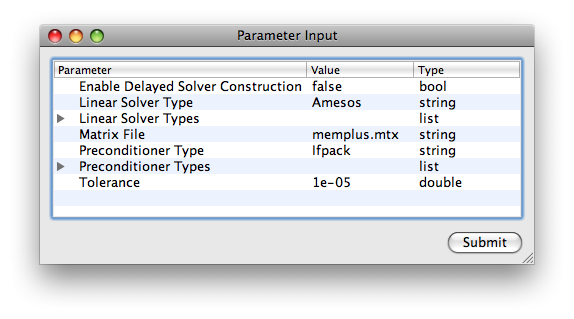
\includegraphics[scale=0.5]{graphics/treeview}
		\caption{The end result of the initial Optika development}
	\end{figure}

\section{Advanced Features}
With the basic framework in place, we were now able to move on to more advanced features. As these advanced features
were developed various refactorings were made to the already existing code in order to support these new features.

	\subsection{Validators}
	One of the goals of Optika is to make life easier for the end-user. It's not enough to simply give the end-user information, it must
	be conveyed in a meaningful way. Validators are a great way of informing an end-user what the valid set of values for a particular parameter are.
	Teuchos ParameterLists already came with built in validator functionality, but the default validators that were available
	were sorely lacking in capability. Three initial sets of validators were created to help deal with the short comings of
	the available validator classes:
	\begin{description}
		\item[EnhancedNumberValidators] allowed for validating various number types. EnhancedNumberValidators have the following abilities:
			\begin{itemize}
				\item Set min and max.
				\item Set the step with which the number value is incremented.
				\item Set the precision with which the number value is displayed.
			\end{itemize}
		\item[StringValidator] allowed for a parameter to be designated as only accepting values of type string
		and allowed for specifying a valid list of values.
		\item[ArrayValidators] allowed for all validator types to be applied to an array of values. The validator
		that is applied to each entry in the array is called the prototype validator.
	\end{description}
	A fourth Validator type, a FileNameValidator, was added later. This validator designates a particular string parameter
	as containing a file path and allows the developer to indicate whether or not the file must already exist. Since filenames
	are such an important type of string, it made sense that they would have their own validator.
	
	By interpreting these validators, Optika could either put certain restrictions on the input widget for a parameter or entirely change the
	type of input widget used. For instance: with EnhancedNumberValidators the min, max, step, and precision of the
	EnhancedNumberValidator are all to directly set their corresponding values in the QSpinBox class. But with the FileNameValidator
	a QFileDialog would appear instead of the normal QComboBox or QTextEdit used for string validators.

	\subsection{Dependencies}
	Many times the state of one parameter depends on the state of another. Common inter-parameter dependencies and their requirements include:
	\begin{description}
		\item[Visual Dependencies:] One parameter may become meaningless when another parameter takes on a particular value.
		In this case the end-user no longer needs to be aware of the meaningless parameter and it's best to just remove it from
		their view entirely so they don't potentially become confused. Visual dependencies should allow the developer to express that "if parameter 
		x takes on a particular value, then don't display parameter y to the end-user anymore."
		\item[Validator Dependencies:] Sometimes the valid set of values for one parameter changes if another parameter takes
		on a particular value. Validator Dependencies should allow the developer to express that "if parameter x takes on a particular value, change
		the validator on parameter y."
		\item[Validator Aspect Dependencies:] Sometimes the developer doesn't want to change the validator on a particular parameter, but
		rather just a certain aspect of it. Validator Aspect Dependencies should allow the developer to express that "if parameter x takes on a particular value,
		change this aspect of the validator on parameter y based on the new value of parameter x"
		\item[Array Length Dependencies:] Sometimes the length of an array in a parameter changes based on the value of another parameter.
		Array Length Dependencies should allow the developer to express that "if parameter x changes its value, change the length of the array
		in parameter y based on the new value of parameter x."
	\end{description}

	Coming up with a way for the developer to easily express these concepts was not a simple task. The first problem that had to be solved was how to keep track of all the dependencies.
	They couldn't just be stored in a ParameterList as a class member because of the recursive structure of ParameterLists. Eventually, it was decided that a new data structure called
	a DependencySheet would hold all the dependencies used for a certain ParameterList. Each Dependency would at minimum specify the dependent parameter
	and the dependee parameter. However, a complication arose. Because we wanted dependencies to be able to have arbitrary dependents and dependees, we needed
	a way to uniquely identify the dependee and the dependent. As the ParameterEntry class stood, there was no way of doing this and we didn't want to add this cabaility to the
	ParameterEntry class. The Teuchos package is fundamental to the Trilinos Project and before we started changing it for our purposes we wanted Optika to have a solid footing and
	be absolutely sure that any changes made to Teuchos were actually necessary. We needed to find another way to uniquely identify parameters within a ParameterList.
	
	We decided to use the name of the parameter as the identifier because the accessor functions for a ParamaeterList usually use the parameters name to identify a particular parameter. 
	While within a ParameterList names of parameters are unique, names are not necessarily unique across a set of sublists. Therefore, in order to uniquely identify a 
	parameter and allow dependencies across sublists Optika would need to know both the parameter name and the parent list containing it\footnote{The astute reader will notice 
	that if there are two sublists with different parent lists and each sublist has a parameter with the same name, then Optika will not be able to uniquely identify the 
	dependent and the dependee. Since solving this problem would most likely require a lot of refactoring of code not directly part of the Optika package, we decided to address it
	at a later date.}.  

	So it became that every dependency, along with needing the names of the dependee
	and dependent, also needed their respective parent lists. The DependencySheet also needed the root list which contained all of the dependees and dependents.
	This was so Optika could recursively search for the parameters and their parent sublists (the only way to find them using our method of identification). 
	The following Dependency classes were created to address the use cases above (shown as a hierarchy of classes):
	\begin{description}
		\item[Dependency:] Parent class for all Dependencies.
		\begin{description}
			\item[NumberArrayLengthDepednency:] Changes an array's length.
			\item[NumberValidatorAspectDependency$<$T$>$:] Changes various aspects of an EnhancedNumberValidator.
			\item[ValidatorDependency:] Changes the validator used for particular parameter.
			\begin{description}
				\item[BoolValidatorDependency:]Changes the validator used for a particular parameter based on a boolean value.
				\item[RangeValidatorDependency$<$T$>$:] Changes the validator used for a particular parameter based on a number value.
				\item[StringValidatorDependency:] Changes the validator used for a particular parameter based on a string value.
			\end{description}	
			\item [VisualDependency:] Shows or hides a particular parameter.
			\begin{description}
				\item[BoolVisualDepedency:] Shows or hides a particular parameter based on a boolean value.
				\item[NumberVisualDependency$<$T$>$:] Shows or hides a particular parameter based on a supported number type value.
				\item[StringVisualDependency:] Shows or hides a particular parameter based on a string value.
			\end{description}
		\end{description}
	\end{description}

	Some of these dependencies have fairly novel and robust capabilities. Namely, the NumberArrayLengthDepednency, NumberValidatorAspectDependency, and NumberVisualDependencies
	can all take a pointer to a function as an argument. In the case of the NumberArrayLengthDepednency, this function can be applied to the value of the dependee
	parameter. The return value of this function is then used as the length of the array for the dependent parameter. For NumberValidatorAspectDependencies, the function
	is applied to the dependee value and used to calculate the value of the chosen validator aspect. In the NumberVisualDepenency class, if the function 
	when applied to the dependee value returns a value greater than 0 the dependent is displayed. Otherwise, the dependent is hidden. 

	The algorithm for expressing dependencies in the GUI is as follows:
	\begin{enumerate}
		\item A parameter's value is changed by the end-user.
		\item The Treemodel queries the associated dependency sheet to see whether or not the parameter that changed has any dependents.
		\item If the parameter does have dependents, the Treemodel requests a list of all the dependencies in which the changed
		parameter is a dependee.
		\item For each dependency, the evaluate function is called. The dependency makes any necessary changes to the dependent parameter
		and the Treemodel updates the Treeview with the new data.
		\item If any dependents now have invalid values, focus is given to them and the end-user is requested to change their value to
		something more appropriate.
	\end{enumerate}

The order in which dependencies are evaluated is arbitrary. We have not
tested what happens under the conditions of conflicting dependencies or 
circular dependencies yet. This is an area for further study.

	\subsection{Custom Functions}
	Normally, in Optika the end-user configures the ParameterList, hits submit, the GUI disappears, and the program continues with execution. However,
	an alternative to this work flow was desired. A persistent GUI was needed. The development team added the ability to specify a pointer to a function
	that would be executed whenever the end-user hit submit. The function was required to have the signature \emph{foo(Teuchos::RCP$<$const ParameterList$>$ userParameters)}.

	\subsection{Various Niceties}
	Various niceties were added to the GUI as well. The ability to save and load ParameterLists was added. The Optika GUI class was expanded to allow for
	customization of the window icon and use of Qt Style Sheets to style the GUI. Checks were also added to see if the end-user was trying to exit the GUI without
	saving. In such a case they would be warned and given the option to save their work. Tooltips were added so when ever the end-user hovered over a parameter, it's 
	documentation string would be displayed. Also, the ability to search for a parameter was added.

\section{Waiting For Copyright}
	All of the above features were completed around or shortly after the end of August 2009 and Optika was officially given its name.
	Optika was then submitted for copyright. It took Optika a little over six months to complete copyright.
	Since it was not yet copyrighted, it could not be included in the Trilinos 10 release in October 2009. During the time Optika spend in copyright limbo, 
	little development on Optika was done. Most of development was cleaning up various pieces of code, adding examples, and adding documentation. 
	Finally, in March 2010 Optika completed copyright and was ready to be included in Trilinos. It was released to the public with the Trilinos 10.2 release.

\section{User Feedback}
In the summer of 2010, Optika got it's first user. Dr. Laurie Frink began using Optika to create a GUI for Tramonto.
There had been a previous attempt to build a GUI for Tramonto, but it had been largely unsuccessful

Initial feedback was very positive. Dr. Frink was very impressed with the capabilities of Optika and the ease at which should could construct a
GUI. However, she did have some small initial issues picking up Optika. But most of them arose from the fact she is a C programer and Optika is C++ based.
Her issues were always easily and quickly addressed. Some of her more involved questions even lead to the creation of some great examples. 

For the most part Dr. Frink found Optika to be quite adequate for her purposes. However, she did have one rather major feature request: 
she needed the ability to specify multiple dependents and in some cases even multiple dependees. This was quite a task and required a 
large reworking of the Dependency part of the framework. 

Adding support for multiple dependents was fairly trivial. Instead of specifying a single dependent to the constructor of a Dependency, a list
of Parameters was now passed. If the developer only needed one dependent then he/she could just pass a list of length one. This simple
list worked in the case of all the dependents having the same parent list. If they had different parent lists, then a more complex 
data structure which mapped parameters to parent lists would be used. Convenience constructors were also made for simple cases where
just one dependent was needed. The algorithm used for evaluating dependencies changed very little with these modifications. The only addition
needed was an extra loop for evaluating each dependent in a dependency for a given dependee.

Adding support for multiple dependents was much harder. There was actually only 
one specific use case where multiple dependents were needed or even appropriate 
for that matter. Dr.
Frink needed the ability to test the condition of multiple parameters to determine whether or not a particular parameter should be displayed.
So a new VisualDependency class called ConditionVisualDependency was created. ConditionVisualDependencies evaluated a condition object to
determine the whether or not a set of dependents should be hidden or shown. The set of condition classes created are as follows (shown as a hierarchy of classes):
\begin{description}
	\item[Condition]: Parent class of all conditions.
	\begin{description}
		\item[ParameterCondition]: examines the value of a particular parameter and evaluates to true or false accordingly. Types of ParameterConditions include:
		\begin{description}
			\item[BoolCondition:] examines boolean parameters.
			\item[NumberCondition$<$T$>$:] examines number parameters.
			\item[StringCondition:] examines string parameters.
		\end{description}
		\item[BinaryLogicalCondition:] examines the value of two or more conditions passed to it and evaluates to true or false accordingly. Types of BinaryLogicalConditions include:
		\begin{description}
			\item[AndCondition:] returns the equivalent of performing a logical AND on all conditions passed to it.
			\item[EqualsCondition:] returns the equivalent of performing a logical EQUALS on all conditions passed to it.
			\item[OrCondition:] returns the equivalent of performing a logical OR on all conditions passed to it.
		\end{description}
		\item[NotCondition:] examines the value of one condition passed to it and evaluates to the opposite of what ever that condition evaluates.
	\end{description}
\end{description}
Through the recursive use of BinaryLogicalConditions the developer can now chain together an arbitrary amount of dependents.

ConditionVisualDependencies are the only dependencies which allow for multiple dependents. So while support was added for multiple dependents at the
Dependency parent class level, ConditionVisualDependency is the only class which actually implements the functionality. In the case of multiple dependents the algorithm
for evaluating dependencies didn't need to change at all.

\section{Serialization}
The next step was to make Optika's dependencies, conditions, and validators
 serializable. In addition, we needed to make the parameter serialization more 
robust. The hope was that by doing this we would allow the application 
developer to specify the majority of their application via XML, instead of the 
more cumbersome source-code solution. After some consulting with Roscoe 
Bartlett, the following model was decided on:
\begin{itemize}
	\item Each different type of condition, dependency, parameter, and validator
		 would have
		it's own associated XMLConverter. All the dependency converters would 
		sub-class a DepenencyXMLConverter super-class, all the condition converters
		would sub-class a ConditionXMLConverter super-class, etc. These converters
		would be able to convert back-and-forth from object and XML.
	\item A psuedo-database class would be created for each set of converters. All
	converters would be obtained by calling a getConverter() function whose 
	parameter would either be a object to convert, or
	and XML tag to convert. The getConverter() function would then return an
	appropriate converter that would allow the object to be converted to and from
	XML or vice versa.
\end{itemize}
This model has the benefit of being extendible If new object 
types are created, or even if the user desires to create their own types,
this model will easily accommodate such additions. A new converter class just
has to be created. 

The summer of 2010 was spent developing the converters for 
the standard conditions, dependencies, parameters, and validators. Also,
we changed from the system of using a parent ParameterList and Parameter name
to identify specific parameters. We now used pointers, which guaranteed a unique
identification of a specific parameter. This was done for two reasons: it was 
the only good way to make serialization possible, and we determined that it was
absolutely necessary for users to be able to uniquely identify parameters.
All these changes resulted in a rather large effort that added a lot of new
code. In addition, new tests had to be developed for this large addition of 
functionality. By September we were basically done with only a few loose ends.
These were taken care of over the next few months.


\section{Future Development}
There are several main development goals for Optika in the near future. 
\begin{itemize}

\item Dr. Frink has submitted several requests for new functionality. Most 
importantly she has identified the need for users to be able to edit two
dimensional arrays. We are currently in the process of adding this 
functionality. She would also like to be able to specify a label to use for
each entry in an array along with a few other niceties.

\item We would like to develop a stand-alone version of Optika. The development team believes that the potential audience for Optika is much 
larger than just the user base of Trilinos. However, creating a stand-alone version presents the problem of keeping source code consistent between
the Optika that exists in Trilinos and the stand-alone version. This is an issue that we will need to make sure to address.

\item We would like to create a single Optika based executable that acts as a generic ParmaterList configurator. It would take in a ParameterList in
XML format, allow the user to configure the ParameterList, and then either output the entire ParameterList again with the new settings or output
a ParameterList only containing the parameters that were changed. We think this will be useful because it will enable end-users to utilize
Opitka without requiring the program their using to implement Optika support (just ParameterList support).

\item We need to further investigate what happens when dependencies conflict
or become circular. Right now the behavior of Optika under such conditions
is unknown.

\end{itemize}

\section{Conclusions}
It is difficult to tell if Optika has met it's initial goals yet. As of the writing of this paper, Optika only has one user. Hopefully, by continuing to do
further development and evangelization it's user base can grow. This will then allow us to see if we truly are meeting the needs of the scientific community.
Based on early use of Optika by Dr. Frink we believe that Optika is indeed robust enough to meet most of the community's needs but we can't say for sure
until we have more user testing.




%    \chapter{A Long Chapter}\label{sec:long}
%$	    We need a long chapter to test full-page formatting. Therefore,
    we switch to the ancient language of Latin.

    %
% Generated by http://www.lipsum.com
% I could have used the LaTeX package lipsum.sty, but it is not present in all
% LaTeX distributions and would make the examples less portable.
%
Lorem ipsum dolor sit amet, consectetuer adipiscing elit. Maecenas ante augue, dictum ut, scelerisque vitae, sagittis vel, velit. Curabitur velit. Curabitur eleifend eleifend felis. Curabitur purus. Nunc aliquet felis a pede. Suspendisse dictum consequat nunc. In accumsan. Sed sit amet diam. Aliquam rhoncus, orci non sodales suscipit, libero risus condimentum lacus, vitae laoreet velit purus ac est. Etiam id sem eu arcu pellentesque rhoncus. Quisque feugiat est at elit lacinia vestibulum. Integer eget nisl sed diam sodales egestas.

Quisque risus libero, pellentesque ac, iaculis a, pulvinar quis, leo. Cras sapien erat, lacinia sit amet, accumsan porta, bibendum malesuada, nulla. Suspendisse non lorem. Sed pellentesque nulla id nisl. In hac habitasse platea dictumst. Ut nec sem. Proin interdum fringilla felis. Aenean lacus. Quisque nisi. Aliquam congue venenatis purus. Vestibulum ante ipsum primis in faucibus orci luctus et ultrices posuere cubilia Curae; Suspendisse a nunc.

Nunc lobortis. Aliquam ultricies volutpat felis. Nulla nisi tellus, ultrices vel, sodales in, lacinia at, leo. Fusce odio turpis, mattis nec, semper ut, aliquam nec, odio. Sed tristique lacus eget arcu. In at elit. Duis semper, est ut sagittis tempor, risus arcu mattis ligula, quis posuere velit ipsum a neque. Proin mattis, urna vehicula tempus placerat, nisl tortor pharetra dolor, nec luctus orci nisi a ante. Ut a lectus at nulla ultricies congue. Ut rhoncus, purus in malesuada rhoncus, nisi ante laoreet lectus, eget volutpat dui nunc ac metus. Sed dignissim faucibus elit. Vestibulum cursus nonummy mauris. Vestibulum dapibus neque eu ligula. Ut scelerisque urna ut orci tincidunt volutpat. Aliquam ipsum purus, eleifend sed, nonummy non, dapibus vel, metus. Class aptent taciti sociosqu ad litora torquent per conubia nostra, per inceptos hymenaeos.

Ut vitae mauris. Aenean diam. Nam euismod massa bibendum orci. Proin sed arcu. Phasellus commodo lacus. Nunc sit amet dolor eget arcu iaculis congue. Sed volutpat, dolor nec porta facilisis, purus mi euismod lacus, sed pharetra magna arcu id dolor. Vestibulum a purus nec nisl varius facilisis. Sed semper mattis lorem. Suspendisse tellus dolor, tincidunt fermentum, imperdiet eu, ultrices et, massa. Nulla facilisi. Nulla rhoncus. Ut vestibulum quam feugiat quam. Aliquam nisi. Vivamus facilisis euismod ipsum. Nunc suscipit semper felis. Nunc non metus. Vestibulum ante ipsum primis in faucibus orci luctus et ultrices posuere cubilia Curae;

Maecenas posuere rutrum odio. Curabitur dolor quam, semper sed, malesuada eu, sagittis eu, erat. Vestibulum facilisis, ipsum vitae venenatis consectetuer, ipsum nibh scelerisque lacus, quis nonummy elit augue et lectus. Fusce ut dolor et ligula laoreet commodo. Phasellus ornare. Aliquam erat volutpat. Ut sapien leo, auctor vel, placerat vel, pretium quis, libero. Integer tempus interdum tellus. Vestibulum posuere, mi ultricies ullamcorper ornare, dolor nunc condimentum tellus, et commodo neque tellus at mi. Aliquam porttitor, tortor eu interdum malesuada, justo nisl feugiat lacus, eu venenatis augue tortor sit amet arcu. Maecenas quis enim. Mauris fringilla diam. Maecenas vitae metus a felis ullamcorper vestibulum. Suspendisse potenti. Etiam sit amet elit. Ut iaculis risus in odio.

Quisque porttitor, velit at consectetuer pretium, nibh lacus dignissim erat, id imperdiet tellus lectus vel sapien. Integer varius dignissim urna. Vestibulum elementum lobortis lorem. Morbi vel metus in risus consectetuer facilisis. Quisque ac purus eget ipsum interdum semper. Suspendisse blandit, nisi in mattis condimentum, elit sem tempus dui, eu convallis mi dolor in dui. Nunc vehicula eros in diam. Sed lectus velit, varius ut, posuere eget, lacinia a, augue. Suspendisse odio lectus, tincidunt porttitor, porttitor vitae, rhoncus id, turpis. Sed quam. Duis tortor tortor, ultrices ut, imperdiet a, convallis a, magna. Donec pellentesque sapien vitae elit. Fusce egestas eleifend velit. Pellentesque habitant morbi tristique senectus et netus et malesuada fames ac turpis egestas.

Proin ac sapien. Aenean tincidunt ante aliquet tortor. In non elit nec tortor pharetra pretium. Nulla facilisi. Maecenas pulvinar odio in libero. Nam tincidunt nulla et dui. Nunc in eros nec dolor congue varius. Suspendisse euismod. Aliquam nulla nibh, vulputate in, molestie ut, suscipit quis, orci. Ut feugiat sapien id velit. Nullam rutrum, enim non dictum posuere, nulla diam faucibus risus, vel suscipit tellus nisi nec libero. Nullam scelerisque vestibulum sem.

Sed ultrices ligula vel lacus. Donec elit felis, venenatis volutpat, varius eu, placerat cursus, sem. Nullam non felis quis enim laoreet dictum. Nulla in nisl at erat pretium facilisis. Vestibulum sed ante. In hac habitasse platea dictumst. Aenean lobortis ullamcorper ante. Aenean at magna. Etiam viverra erat id augue. Morbi purus. Sed congue. Integer sit amet enim vel sapien ullamcorper auctor. Phasellus neque sapien, cursus sit amet, pharetra ac, mollis non, nibh. Ut risus orci, dignissim eu, feugiat sit amet, ullamcorper sit amet, tortor. Nunc ac ligula ut libero fermentum tincidunt. Morbi lorem metus, bibendum ut, aliquet at, tristique vulputate, nisl. Duis risus turpis, bibendum in, faucibus cursus, eleifend sit amet, erat. Donec elit purus, facilisis nec, vulputate non, gravida et, eros. Curabitur porttitor sapien ac magna. Donec cursus.

Cras sodales posuere pede. Lorem ipsum dolor sit amet, consectetuer adipiscing elit. Donec id nisi eu erat tempus ornare. Ut diam magna, bibendum sit amet, porttitor tempor, malesuada non, tellus. Duis iaculis gravida ante. Morbi dapibus elementum orci. Donec eget metus. Curabitur varius tortor condimentum nunc. In arcu. Nam ante justo, porta sed, pellentesque vitae, tristique in, metus. Nam ultricies nulla quis tellus. Donec egestas enim et dolor. In ornare ligula et eros.

Proin augue ligula, dictum non, viverra vitae, convallis sed, ipsum. Maecenas vitae justo. Lorem ipsum dolor sit amet, consectetuer adipiscing elit. Aliquam erat volutpat. Aenean eget ligula. Nullam id dui eu lacus euismod iaculis. Nulla erat purus, convallis ac, ullamcorper a, vestibulum id, erat. Sed pulvinar consectetuer neque. Nulla lobortis. Nulla congue, sapien in hendrerit rhoncus, est sem dignissim mauris, non nonummy nunc justo volutpat velit. Quisque suscipit risus a ipsum mattis viverra. Pellentesque habitant morbi tristique senectus et netus et malesuada fames ac turpis egestas. Vestibulum ante ipsum primis in faucibus orci luctus et ultrices posuere cubilia Curae; Fusce libero dolor, aliquam vel, varius id, faucibus sollicitudin, massa.

Proin iaculis semper ligula. Pellentesque malesuada, neque sit amet ornare mattis, augue lacus auctor tellus, quis porttitor felis sapien a nibh. In sed orci. Pellentesque congue purus sit amet urna. Proin tincidunt molestie nibh. Nulla et dui ac turpis venenatis ullamcorper. Nunc at nisl. Pellentesque habitant morbi tristique senectus et netus et malesuada fames ac turpis egestas. Cum sociis natoque penatibus et magnis dis parturient montes, nascetur ridiculus mus. Sed magna. Curabitur gravida, metus id semper interdum, dui orci ullamcorper massa, congue ornare mauris lectus rhoncus mi. Integer justo ante, sollicitudin tempor, egestas sit amet, egestas eu, eros. Etiam leo. Integer tristique velit nec nunc.

Nulla ac nibh id nunc volutpat ultrices. Lorem ipsum dolor sit amet, consectetuer adipiscing elit. Praesent a arcu. Suspendisse blandit justo eu justo. Nunc turpis metus, iaculis eget, molestie eu, egestas hendrerit, nibh. Sed elementum placerat metus. Cras pretium turpis non ipsum. Duis in libero. Praesent ut elit eu magna tempus rhoncus. Nunc consectetuer quam ac orci. In nulla.

Donec porta turpis a velit. Donec accumsan. Pellentesque augue magna, cursus sed, elementum eget, cursus id, enim. Duis purus. Suspendisse tristique. Quisque condimentum. Quisque tristique lacus vitae nulla. Nunc nibh velit, gravida et, placerat nec, feugiat sed, ante. Phasellus nisi. Aenean auctor pede at leo. Nullam semper fringilla dui. Quisque est. Suspendisse dolor sem, euismod ac, tempor vitae, nonummy id, felis. Mauris eu tellus. Morbi rhoncus. Cum sociis natoque penatibus et magnis dis parturient montes, nascetur ridiculus mus. Nam sed nisi. Fusce ac sapien sit amet arcu venenatis facilisis. Proin faucibus pharetra risus.

Sed varius elit vitae urna. Ut at felis. Phasellus euismod metus a ante. Suspendisse eu massa. Nullam bibendum dui pulvinar turpis. Mauris lacinia odio id augue. Morbi ligula. Nulla ac massa. Nullam vel arcu. Pellentesque iaculis, tellus et convallis condimentum, erat diam viverra nibh, eget pellentesque mauris lorem faucibus neque.

Curabitur tincidunt, dui ac dictum iaculis, enim magna porttitor orci, quis ullamcorper enim magna commodo justo. Aliquam ut quam in velit porta consequat. Suspendisse potenti. Nunc cursus rutrum eros. Curabitur varius molestie massa. Fusce accumsan fringilla sem. Pellentesque habitant morbi tristique senectus et netus et malesuada fames ac turpis egestas. In hac habitasse platea dictumst. Pellentesque risus nisl, tincidunt sed, sodales ac, interdum ac, diam. In purus ipsum, porttitor feugiat, viverra ac, mattis eget, ligula. Sed bibendum libero in metus. Morbi ornare. Donec libero justo, fringilla vitae, mollis sit amet, molestie ut, mauris. Morbi vel dolor. Donec at elit eget metus semper pharetra. Morbi est massa, volutpat ut, viverra varius, sagittis blandit, sapien. Sed dapibus. Pellentesque erat. Nullam hendrerit. Vestibulum vel diam in tortor consectetuer volutpat.

Quisque accumsan, elit quis sodales pellentesque, sapien metus consequat enim, et commodo leo nulla in elit. Donec varius. Donec ut risus. Donec quis lacus quis nisi congue consectetuer. In sed odio. Duis nulla sem, ullamcorper ac, suscipit dignissim, suscipit vel, turpis. Fusce suscipit. Maecenas in augue non felis fermentum luctus. Aenean sem. Etiam in leo sit amet tortor malesuada auctor. Curabitur quis massa. Maecenas aliquam lectus. Maecenas sit amet augue. Sed sem elit, egestas vitae, condimentum suscipit, elementum et, nulla. Lorem ipsum dolor sit amet, consectetuer adipiscing elit. Nam dignissim tristique velit.

Pellentesque dui elit, tristique non, cursus a, elementum sed, magna. Ut eu augue. Maecenas scelerisque lectus vel enim. Vivamus eu mauris. Phasellus venenatis. Maecenas egestas. Phasellus ac purus. Sed vel dui. Nam consectetuer venenatis lacus. Morbi ullamcorper, urna ac viverra tempor, urna dui imperdiet dui, sit amet hendrerit elit nisi ac lorem. Nullam gravida diam ut tellus. Aenean quam tortor, condimentum ac, commodo non, pharetra in, elit. Mauris tincidunt, orci sit amet lacinia varius, diam tortor dapibus tellus, id scelerisque quam magna pharetra libero. Curabitur aliquet, ante sit amet ornare volutpat, urna ipsum dictum ipsum, at ullamcorper ligula arcu eget leo.

Ut libero lorem, condimentum nec, rhoncus id, vestibulum a, nisl. Cras hendrerit euismod sapien. Sed lectus ipsum, vehicula et, luctus vitae, venenatis at, magna. Ut nec nisl in quam facilisis tincidunt. Fusce enim purus, pellentesque vitae, molestie ut, dapibus in, eros. Integer eu turpis vel pede volutpat posuere. Nam porttitor suscipit metus. Curabitur mollis, quam quis porttitor nonummy, libero ante pulvinar magna, a bibendum massa erat nec sapien. Donec ac turpis. Suspendisse elit nisi, ultrices ut, fringilla sed, vestibulum suscipit, mauris. Cum sociis natoque penatibus et magnis dis parturient montes, nascetur ridiculus mus. Phasellus dictum aliquam lacus. Praesent in erat quis nunc consectetuer dictum. Morbi dignissim, turpis ut varius pharetra, tellus lectus rutrum lacus, bibendum iaculis velit nulla ac orci. Etiam gravida nibh eget massa. Sed elementum convallis purus. Duis tincidunt feugiat lacus. Donec id enim nec enim ullamcorper condimentum. Suspendisse urna.




%    \chapter{Conclusion}
%	    Of course, no report would be complete without some conclusions.
    This section is where they would go, if we had any.


    \nocite{*}


    % ---------------------------------------------------------------------- %
    % References
    %
    \clearpage
    % If hyperref is included, then \phantomsection is already defined.
    % If not, we need to define it.
    \providecommand*{\phantomsection}{}
    \phantomsection
    \addcontentsline{toc}{chapter}{References}
    \bibliographystyle{plain}
    \bibliography{OptikaSANDReport}


    % ---------------------------------------------------------------------- %
    %
    %\appendix
    %\chapter{Historical Perspective}
	%    This is an example of an appendix.

    If we follow~\cite{Sand98-0730} strictly, we would have to have
    a separate bibliography section for each appendix.  The style
    file doesn't provide that, but it can be done using the {\tt
    bibunits} and {\tt chapterbib} packages.

    If there are many subsections in an appendix, it should also
    have its own table of contents. Again, the SAND report class
    file does not provide that functionality.

    \ifthenelse{\boolean{reportSAND}}   {
	\section{The Past a Long Time Ago}
    }{
	\subsection{The Past a Long Time Ago}
    }
	This is where we talk about things so old nobody can verify
	them. We are safe.

    \ifthenelse{\boolean{reportSAND}}   {
	\section{The Past More Recently}
    }{
	\subsection{The Past More Recently}
    }
	Now we have to be a little bit more careful, since records
	exist from that time, and some people still alive actually
	lived back then.



    %\chapter{Some Other Appendix}
	%    Just to show what a second Appendix would look like. It contains
    a table. Each appendix is supposed to be self-contained, so
    tables and figures are not supposed to show up in the main
    table of contents. There can be a separate table of contents
    for each appendix.

    \begin{table}[ht]
	\centering
	\caption{A small table}
	\bigskip

	\begin{tabular}{|c|c|}
	    \hline
		A & B  \\ \hline
		C & D  \\ \hline
	\end{tabular}
	\label{tab3}
    \end{table}

    \begin{figure}[ht]
	\centering
	\begin{picture}(50,50)(0,0)
	    \put(25,25){\circle{1}}
	    \put(25,25){\circle{5}}
	    \put(25,25){\circle{10}}
	    \put(25,25){\circle{15}}
	    \put(25,25){\circle{20}}
	    \put(25,25){\circle{25}}
	    \put(25,25){\circle{30}}
	    \put(25,25){\circle{35}}
	    \put(25,25){\circle{40}}
	    \put(25,25){\circle{45}}
	    \put(25,25){\circle{50}}
	\end{picture}
	\caption{Dizzy yet?}
	\label{fig4}
    \end{figure}


    % \printindex

    %
% This is an example of how to create the distribution page. Some
% distributions are required by Sandia; e.g. the housekeeping copies.
% Depending on the type of report; e.g. CRADA, Patent Caution, etc.
% additional distribution lines may have to be added. See the
% "Guide for Preparing SAND Reports"
%
% SANDdistribution takes CA or NM as an optional argument. If given,
% the approrpiate housekeeping copies are inserted autmatically.
% Inside the SANDdistribution environment, several commands can be used
% insert the distributions for CRADA, LDRD, etc. See example below.
%
% You can leave the CA or NM option off and not use any of the SANDdist*
% commands. This will allow you to create a distribution list manually.
%
\begin{SANDdistribution}[NM]
    % Housekeeping copies necessary for every unclassified report:
    % \SANDdistCRADA	% If this report is about CRADA work
    % \SANDdistPatent	% If this report has a Patent Caution or Patent Interest
    % \SANDdistLDRD	% If this report is about LDRD work

    % Some external Addresses
    \SANDdistExternal{1}{An Address\\ 99 $99^{th}$ street NW\\City, State}
    \SANDdistExternal{3}{Some Address\\ and street\\City, State}
    \SANDdistExternal{12}{Another Address\\ On a street\\City, State\\U.S.A.}
    \bigskip


    % The following MUST BE between the external and internal distributions!
    % \SANDdistClassified % If this report is classified


    % Internal Addresses
    \SANDdistInternal{1}{1319}{Rolf Riesen}{1423}
    \SANDdistInternal{1}{1110}{Another One}{01400}

    % Example of a mail channel use (instead of a mail stop)
    \SANDdistInternalM{1}{M9999}{Someone}{01234}

\end{SANDdistribution}


    % The second printing
    \begin{SANDreDistribution}
	% Some external Addresses
	\SANDdistExternal{1}{An Address\\ 99 $99^{th}$ street NW\\City, State}
	\SANDdistExternal{3}{Some Address\\ and street\\City, State}
	\SANDdistExternal{12}{Another Address\\ On a street\\City, State\\U.S.A.}
	\bigskip


	% Internal Addresses
	\SANDdistInternal{1}{1319}{Rolf Riesen}{1423}

	% Example of a mail channel use (instead of a mail stop)
	\SANDdistInternalM{1}{M9999}{Someone}{01234}
    \end{SANDreDistribution}

    % The third printing
    \begin{SANDreDistribution}
	\SANDdistInternal{1}{1319}{Rolf Riesen}{01423}
    \end{SANDreDistribution}

    % The fourth printing
    \begin{SANDreDistribution}
	\SANDdistInternal{1}{1319}{Rolf Riesen}{1423}
    \end{SANDreDistribution}

\end{document}
